\section{Enhancing SOM for socially connected data}
\begin{frame}{Homophilic SOM}
  \begin{figure}
    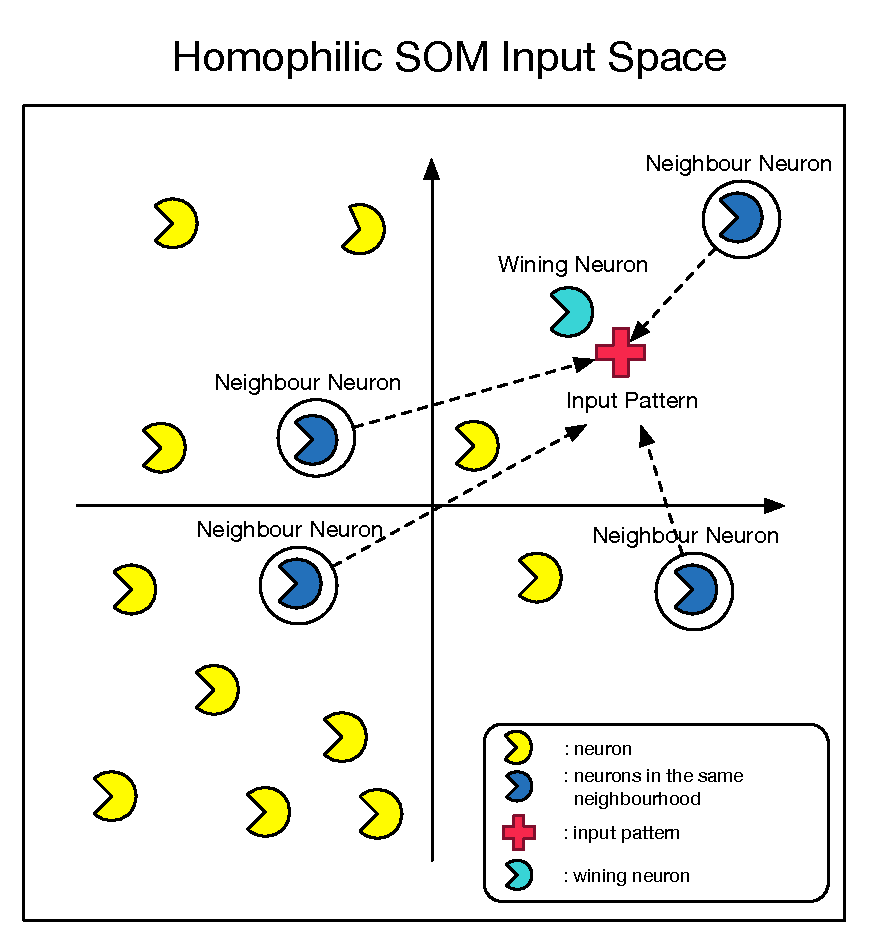
\includegraphics[width=0.5\textwidth]{images/homophilic_input_space.pdf}
  \end{figure}
\end{frame}

\begin{frame}{Homophilic SOM}
  \begin{figure}
    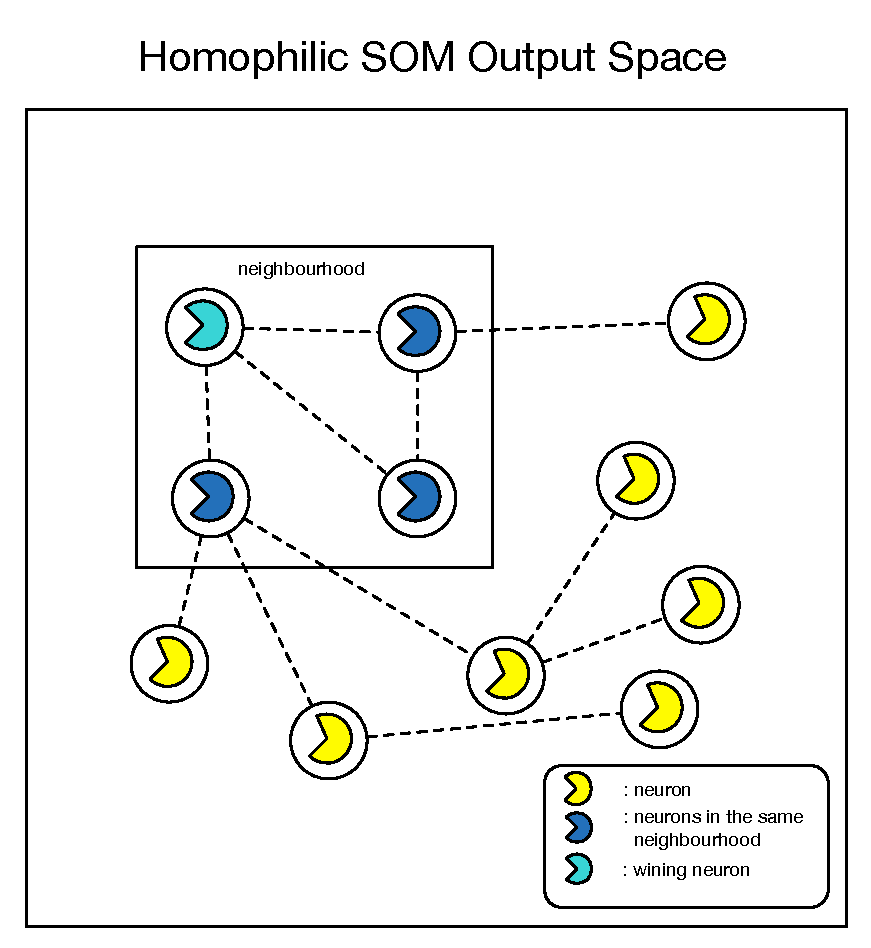
\includegraphics[width=0.5\textwidth]{images/homophilic_outputspace.pdf}
  \end{figure}
\end{frame}

\begin{frame}{SOM Framework}
  \textbf{Why develop another SOM library? }
  \begin{itemize}
    \item Current SOM libraries don't allow the neighborhood function to be defined before training. 
    \item A lot of customizations to the SOM algorithm where made, and each has its own code. 
    \item SOM implementations on higher level languages rely on C. 
    \item Easy to test new SOM approaches.
  \end{itemize}
\end{frame}

\begin{frame}{Testing SOM Framework}
  \textbf{Using the SOM framework to train a SOM to identify different colors:}
  \begin{figure}
    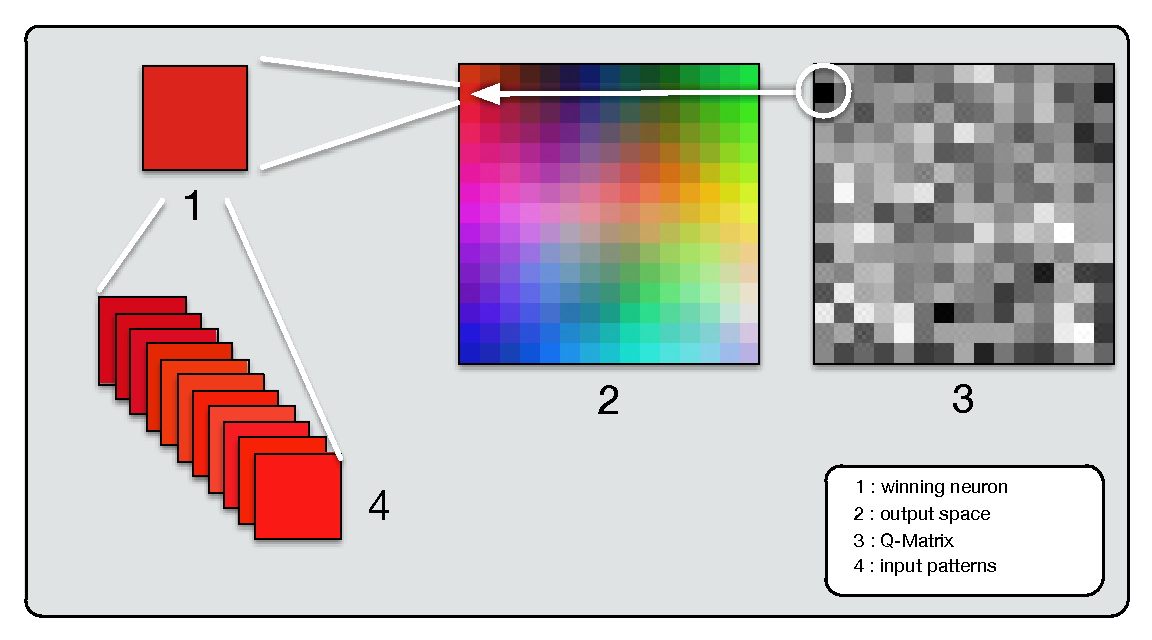
\includegraphics[width=1\textwidth]{images/som_trainned.pdf}
  \end{figure}
\end{frame}

\begin{frame}{Homophilic SOM Implementation}
  \begin{itemize}
    \item On top of the SOM framework.
    \item Changed the Output Space class, which was no longer squared.
    \item Everything keeps working as it was supposed to.
  \end{itemize}
\end{frame}

\begin{frame}{Homophilic SOM Results}
  \begin{itemize}
    \item I think I haven't had a segmentation fault in years
    \item Just bought a banana phone at \#bananamarket
    \item Real Software Engineering by @glv via @confreaks. @daviddias you're going to enjoy this (it is not about ruby)
    \item R vrs SAS, interesting debate: 
    \item I'm finding @duckduckgo to be pretty more reliable than google when searching for code. Gonna try it as my default se.
    \item Mind blowing results! Taking Commercial 3DP into the Nano Dimension - \#3DPrinting | @scoopit 
  \end{itemize}
\end{frame}
